\documentclass[12pt,a4paper]{article}

% ─── Page Layout ───────────────────────────────────────────────────────────────
\usepackage[a4paper, margin=0.8in, headheight=14pt]{geometry}

% ─── Fonts (XeLaTeX) ───────────────────────────────────────────────────────────
\usepackage{fontspec}
\usepackage{unicode-math}
\setmainfont{TeX Gyre Pagella}
\setmonofont[Scale=0.88]{TeX Gyre Cursor}
\setmathfont{Latin Modern Math}

% ─── Packages ──────────────────────────────────────────────────────────────────
\usepackage{xcolor}
\usepackage{colortbl}
\usepackage{titlesec}
\usepackage{enumitem}
\usepackage{tabularx}
\usepackage{longtable}
\usepackage{booktabs}
\usepackage{array}
\usepackage{amsmath}
\usepackage{tikz}
\usetikzlibrary{shapes.geometric, arrows.meta, positioning, calc, fit, decorations.pathreplacing, patterns}
\usepackage{tcolorbox}
\tcbuselibrary{skins, breakable}
\usepackage{hyperref}
\usepackage{fancyhdr}
\usepackage{graphicx}
\usepackage{microtype}
\hyphenpenalty=10000
\exhyphenpenalty=10000
\sloppy
\usepackage{caption}
\usepackage{setspace}
\usepackage{multirow}
\usepackage{tocloft}

% ─── Q&A helper ────────────────────────────────────────────────────────────────
\newcommand{\Q}[1]{\textbf{#1}\par\noindent\ignorespaces}

% ─── Colour Palette ────────────────────────────────────────────────────────────
\definecolor{myred}{RGB}{196,30,58}
\definecolor{mydark}{RGB}{30,30,50}
\definecolor{mygreen}{RGB}{14,120,80}
\definecolor{myteal}{RGB}{0,130,140}
\definecolor{myamber}{RGB}{180,100,0}
\definecolor{mypurple}{RGB}{100,30,160}
\definecolor{mygray}{RGB}{246,247,249}
\definecolor{mgframe}{RGB}{180,185,200}
\definecolor{watermark}{RGB}{145,150,170}
\definecolor{hdrred}{RGB}{250,232,235}
\definecolor{hdrgreen}{RGB}{220,244,233}
\definecolor{hdrteal}{RGB}{220,242,244}
\definecolor{hdramber}{RGB}{253,242,215}
\definecolor{hdrpurple}{RGB}{238,228,255}
\definecolor{hdrgray}{RGB}{238,240,245}

% ─── Section Formatting ────────────────────────────────────────────────────────
\titleformat{\section}
  {\large\bfseries\color{myred}}{\thesection.}{0.5em}{}
  [\vspace{1pt}{\color{myred}\rule{\linewidth}{0.8pt}}]
\titleformat{\subsection}
  {\normalsize\bfseries\color{myteal}}{\thesubsection}{0.5em}{}
\titlespacing*{\section}{0pt}{18pt}{7pt}
\titlespacing*{\subsection}{0pt}{11pt}{4pt}

% ─── Paragraph ─────────────────────────────────────────────────────────────────
\setlength{\parindent}{0pt}
\setlength{\parskip}{4pt}

% ─── TOC Styling ───────────────────────────────────────────────────────────────
\renewcommand{\cfttoctitlefont}{\large\bfseries\color{myred}}
\renewcommand{\cftaftertoctitle}{\par\noindent{\color{myred}\rule{\linewidth}{0.8pt}}}
\setlength{\cftbeforetoctitleskip}{0pt}
\setlength{\cftaftertoctitleskip}{6pt}
\renewcommand{\cftsecfont}{\normalsize\bfseries\color{mydark}}
\renewcommand{\cftsecpagefont}{\normalsize\bfseries\color{mydark}}
\renewcommand{\cftsecleader}{\cftdotfill{\cftdotsep}}
\setlength{\cftbeforesecskip}{7pt}
\renewcommand{\cftsubsecfont}{\small\color{mydark}}
\renewcommand{\cftsubsecpagefont}{\small\color{mydark}}
\setlength{\cftbeforesubsecskip}{3pt}
\setlength{\cftsubsecindent}{1.4em}

% ─── Table helpers ─────────────────────────────────────────────────────────────
\renewcommand{\arraystretch}{1.45}
\setlength{\tabcolsep}{6pt}
\arrayrulecolor{mydark}
\newcolumntype{B}[1]{>{\small\bfseries\raggedright\arraybackslash}m{#1}}
\newcolumntype{Y}{>{\small\raggedright\arraybackslash}X}
\renewcommand{\tabularxcolumn}[1]{m{#1}}

% ─── Header / Footer ───────────────────────────────────────────────────────────
\pagestyle{fancy}
\fancyhf{}
\fancyhead[L]{\small\color{myred}\textbf{BS-B401}\;\color{mydark}--- Biology for Engineers}
\fancyhead[R]{\small\color{myteal}\textbf{Module 4 Notes}}
\fancyfoot[C]{\small\color{mydark}\thepage}
\fancyfoot[R]{\small\color{watermark}\textit{\copyright\ Biraj Sarkar (CGEC)}}
\renewcommand{\headrulewidth}{0.5pt}
\renewcommand{\footrulewidth}{0.3pt}

% ─── Hyperref ──────────────────────────────────────────────────────────────────
\hypersetup{
  colorlinks=true, linkcolor=myteal, urlcolor=myteal,
  pdfauthor={Biraj Sarkar (CGEC)},
  pdftitle={BS-B401 --- Module 4 Notes: Biomolecules}
}

% ─── tcolorbox styles ──────────────────────────────────────────────────────────
\tcbset{
  tikzbox/.style={
    colback=mygray, colframe=mgframe, boxrule=0.6pt, arc=4pt,
    left=8pt, right=8pt, top=6pt, bottom=6pt,
    colbacktitle=mgframe, coltitle=mydark, fonttitle=\small\bfseries
  },
  defbox/.style={
    colback=hdrgreen, colframe=mygreen, boxrule=0.8pt, arc=4pt,
    left=9pt, right=9pt, top=6pt, bottom=6pt,
    colbacktitle=mygreen, coltitle=white, fonttitle=\small\bfseries
  },
  formulabox/.style={
    colback=hdrteal, colframe=myteal, boxrule=0.8pt, arc=4pt,
    left=9pt, right=9pt, top=7pt, bottom=7pt,
    colbacktitle=myteal, coltitle=white, fonttitle=\small\bfseries
  },
  examplebox/.style={
    colback=hdramber, colframe=myamber, boxrule=0.8pt, arc=4pt,
    left=9pt, right=9pt, top=6pt, bottom=6pt,
    colbacktitle=myamber, coltitle=white, fonttitle=\small\bfseries
  },
  masonbox/.style={
    colback=hdrpurple, colframe=mypurple, boxrule=0.8pt, arc=4pt,
    left=9pt, right=9pt, top=6pt, bottom=6pt,
    colbacktitle=mypurple, coltitle=white, fonttitle=\small\bfseries
  },
  exambox/.style={
    colback=hdrpurple, colframe=mypurple, boxrule=1pt, arc=5pt,
    left=10pt, right=10pt, top=8pt, bottom=8pt,
    colbacktitle=mypurple, coltitle=white, fonttitle=\bfseries,
    breakable, title after break={\textbf{Frequently Asked / Viva Questions (contd.)}}
  }
}
\tcbset{breakable}
\tcbset{after={\par\color{black}}}

% ─── TikZ styles ───────────────────────────────────────────────────────────────
\tikzset{
  block/.style={rectangle, draw=myteal, fill=hdrteal,
    text width=2.4cm, align=center, minimum height=0.95cm,
    font=\small, rounded corners=3pt, line width=0.7pt},
  redblock/.style={rectangle, draw=myred, fill=hdrred,
    text width=2.4cm, align=center, minimum height=0.95cm,
    font=\small, rounded corners=3pt, line width=0.7pt},
  amberblock/.style={rectangle, draw=myamber, fill=hdramber,
    text width=2.4cm, align=center, minimum height=0.95cm,
    font=\small, rounded corners=3pt, line width=0.7pt},
  sumjunc/.style={circle, draw=myamber, fill=hdramber,
    minimum size=0.62cm, font=\small, line width=0.8pt},
  arrow/.style={-Stealth, thick, color=mydark},
  redarrow/.style={-Stealth, thick, color=myred},
  line/.style={thick, color=mydark}
}

\begin{document}

% ─── Title Page ───────────────────────────────────────────────────────────────
\begin{center}
  {\LARGE\bfseries\color{myred} BS-B401 --- Biology for Engineers}\\[5pt]
  {\normalsize\color{mydark} Semester IV \quad$\bullet$\quad 2L:1T:0P \quad$\bullet$\quad 3 Credits}\\[3pt]
  {\normalsize\color{myteal}\textbf{Module 4 Exam Notes: Biomolecules}}\\[3pt]
  {\small\color{mydark} CGEC \;$|$\; B.Tech ECE (2023--27) \;$|$\; \textit{Biraj Sarkar}}
\end{center}
\vspace{2pt}
\noindent{\color{myred}\rule{\linewidth}{1.5pt}}
\vspace{2pt}

\hypersetup{linkcolor=mydark}
\tableofcontents
\hypersetup{linkcolor=myteal}
\newpage

\section{Biomolecules}
\subsection{Shared building blocks and different structures}
\begin{tcolorbox}[defbox, title={Monomer and polymer}]
A monomer is a small building unit that can be joined to others. A polymer contains repeated or related units connected by covalent bonds. The arrangement, linkage and branching of its building blocks influence function. Most lipids are assembled molecules rather than repeating-chain polymers.
\end{tcolorbox}

\par\vspace{5pt}
\begingroup
\setlength{\extrarowheight}{1pt}
\noindent\begin{tabularx}{\linewidth}{|B{3.1cm}|Y|Y|}
\hline
\textbf{Family} & \textbf{Units and linkage} & \textbf{Biological roles} \\ \hline
Carbohydrates & Monosaccharides joined by glycosidic bonds. & Fuel, storage, recognition and structural support. \\ \hline
Proteins & Amino acids joined by peptide bonds. & Catalysis, transport, signalling and structure. \\ \hline
Nucleic acids & Nucleotides joined by phosphodiester bonds. & Information storage, transfer and some catalysis. \\ \hline
Lipids & Fatty acids, glycerol or other lipid precursors assembled into different families. & Energy storage, membranes and signalling. \\ \hline
\end{tabularx}\par
\endgroup
\subsection{Sugars, starch and cellulose}
\begin{itemize}[leftmargin=*, itemsep=3pt, topsep=4pt]
  \item \textbf{Monosaccharide.} A single sugar unit, such as glucose, ribose or fructose. Glucose is a common metabolic fuel. Ribose is a component of RNA.
  \item \textbf{Disaccharide.} Two sugar units linked by a glycosidic bond. Sucrose contains glucose and fructose.
  \item \textbf{Configuration.} The $\alpha$ and $\beta$ labels distinguish stereochemistry at the anomeric carbon. This difference changes the direction in which glucose units link.
\end{itemize}
\par\vspace{5pt}
\begingroup
\setlength{\extrarowheight}{1pt}
\noindent\begin{tabularx}{\linewidth}{|B{3.1cm}|Y|Y|}
\hline
\textbf{Polysaccharide} & \textbf{Linkages and shape} & \textbf{Function} \\ \hline
Starch: amylose & Mostly linear $\alpha(1\to4)$ glucose chains. Chains can coil. & Plant storage carbohydrate. \\ \hline
Starch: amylopectin & $\alpha(1\to4)$ main chains with $\alpha(1\to6)$ branch points. & Branched component of plant starch. \\ \hline
Cellulose & Linear $\beta(1\to4)$ glucose chains. Adjacent chains associate through hydrogen bonding. & Tough plant cell-wall microfibrils. \\ \hline
\end{tabularx}\par
\endgroup
\begin{tcolorbox}[examplebox, title={Same monomer, different material}]
Starch and cellulose both contain glucose. Human digestive enzymes can hydrolyse the common starch linkages, while humans lack cellulase for the cellulose linkage. The different bond geometry also helps cellulose form extended fibres, making it suitable for support.
\end{tcolorbox}

\subsection{Amino acids and proteins}
An ordinary alpha-amino acid has an alpha carbon attached to an amino group, a carboxyl group, a hydrogen and a side chain $R$. Glycine has $R=\mathrm H$. The side chain affects polarity, charge and interactions.
\begin{enumerate}[leftmargin=*, itemsep=3pt, topsep=4pt]
  \item \textbf{Join.} A peptide bond joins the carboxyl-derived carbon of one residue to the amino-derived nitrogen of the next. In a simplified chemical representation, joining releases water.
  \item \textbf{Read direction.} A protein sequence is conventionally written from the amino (N) terminus to the carboxyl (C) terminus.
  \item \textbf{Fold.} The order and interactions of side chains influence a polypeptide's shape. The resulting structure contributes to function. Module 7 develops the four levels of organisation.
\end{enumerate}
\subsection{Nucleotides and nucleic acids}
\begin{tcolorbox}[defbox, title={Nucleotide}]
A nucleotide contains a nitrogenous base, a pentose sugar and at least one phosphate group. A nucleoside is a base plus sugar. In DNA and RNA, phosphodiester linkages connect the sugars through phosphate groups to form a directional backbone.
\end{tcolorbox}

\par\vspace{5pt}
\begingroup
\setlength{\extrarowheight}{1pt}
\noindent\begin{tabularx}{\linewidth}{|B{3.1cm}|Y|Y|}
\hline
\textbf{Property} & \textbf{DNA} & \textbf{RNA} \\ \hline
Sugar & Deoxyribose. & Ribose. \\ \hline
Bases & A, T, G and C. & A, U, G and C. \\ \hline
Common organisation & Double-stranded helix in cells. & Often single-stranded, with complementary regions folded into local structures. \\ \hline
Typical roles & Stable cellular hereditary information. & Messages, adaptors, structural and catalytic roles. \\ \hline
\end{tabularx}\par
\endgroup
\section{Lipids and the Two-Carbon Unit}
\subsection{Acetyl units, fatty acids and lipid classes}
\begin{itemize}[leftmargin=*, itemsep=3pt, topsep=4pt]
  \item \textbf{Acetyl unit.} Acetyl-CoA carries a two-carbon acetyl group and links carbohydrate, fatty acid and amino acid metabolism.
  \item \textbf{Chain growth.} In fatty-acid synthesis, acetyl-derived building blocks supply two-carbon additions. Malonyl groups provide the elongating units after loss of carbon dioxide.
  \item \textbf{Chain breakdown.} Beta-oxidation shortens many fatty acids, releasing two-carbon acetyl-CoA units.
  \item \textbf{Packing.} Saturated chains have no carbon--carbon double bonds. A cis double bond can kink an unsaturated chain and reduce tight packing. Amphipathic phospholipids organise into bilayers in water.
\end{itemize}
\par\vspace{5pt}
\begingroup
\setlength{\extrarowheight}{1pt}
\noindent\begin{tabularx}{\linewidth}{|B{3.2cm}|Y|Y|}
\hline
\textbf{Lipid class} & \textbf{Structure to recognise} & \textbf{Role} \\ \hline
Triacylglycerol & Three fatty acids esterified to glycerol. & Energy storage. \\ \hline
Phospholipid & A polar phosphate-containing head and hydrophobic regions. & Amphipathic membrane component. \\ \hline
Sterol & A rigid fused-ring structure with a small polar part. & Cholesterol contributes to animal membranes and is a precursor for other compounds. \\ \hline
\end{tabularx}\par
\endgroup
\begin{tcolorbox}[tikzbox, title={Simplified phospholipid bilayer}]
\centering
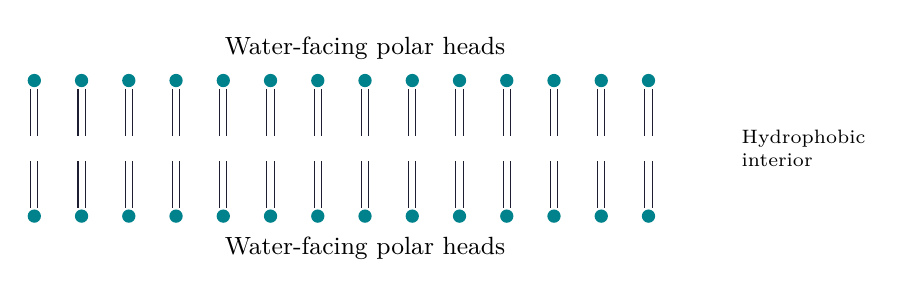
\begin{tikzpicture}[y=0.82cm,every node/.style={font=\small}]
\foreach \x in {0,0.6,...,8.4}{
  \fill[myteal] (\x,1.05) circle (2.4pt);
  \fill[myteal] (\x,-1.05) circle (2.4pt);
  \draw[mydark] ([xshift=-1.3pt]\x,0.92)--([xshift=-1.3pt]\x,0.19)
                 ([xshift=1.3pt]\x,0.92)--([xshift=1.3pt]\x,0.19);
  \draw[mydark] ([xshift=-1.3pt]\x,-0.92)--([xshift=-1.3pt]\x,-0.19)
                 ([xshift=1.3pt]\x,-0.92)--([xshift=1.3pt]\x,-0.19);
}
\node[font=\small] at (4.2,1.55) {Water-facing polar heads};
\node[font=\small] at (4.2,-1.55) {Water-facing polar heads};
\node[anchor=west,align=left,font=\scriptsize] at (8.86,0) {Hydrophobic\\interior};
\end{tikzpicture}\par
\end{tcolorbox}



\subsection{Relate bond chemistry to macromolecular behaviour}
\par\vspace{6pt}
\noindent\begin{tabularx}{\linewidth}{|B{3.2cm}|Y|Y|}
\hline
\textbf{Bond or interaction} & \textbf{Where it matters} & \textbf{Consequence} \\ \hline
Glycosidic bond & Links sugar residues at specified carbon positions. & Changing the linkage can change shape and which enzymes recognise the chain. \\ \hline
Peptide bond & Links the carboxyl-derived carbon of one residue to the amino-derived nitrogen of the next. & Gives a directional polypeptide backbone. \\ \hline
Phosphodiester bond & Joins neighbouring sugars through a phosphate. & Creates a directional, negatively charged nucleic-acid backbone. \\ \hline
Hydrogen bonding & Between cellulose chains, or between complementary bases in DNA. & Helps stabilise a structure without being the covalent linkage along either chain. \\ \hline
\end{tabularx}\par

\begin{tcolorbox}[examplebox, title={Explain reducing and nonreducing sugars}]
A reducing sugar has an anomeric centre that can open to a form with a reactive carbonyl group. In maltose, one anomeric carbon remains free. In sucrose, the glycosidic linkage joins the anomeric carbons of glucose and fructose, leaving neither free. This structural distinction explains why the two disaccharides can behave differently even though both contain two sugar units.
\end{tcolorbox}

\subsection{Use chain direction and unit count correctly}
\begin{itemize}[leftmargin=*, itemsep=2pt]
  \item \textbf{Polypeptide.} A single unbranched chain with $n$ amino-acid residues has $n-1$ peptide bonds. A chain of eight residues therefore has seven such bonds and one N terminus and one C terminus.
  \item \textbf{Nucleic acid.} A single linear strand with $n$ nucleotides contains $n-1$ internucleotide phosphodiester linkages. The two strands of a DNA duplex each have their own backbone.
  \item \textbf{Fat.} A triacylglycerol uses three ester bonds to attach three fatty acids to one glycerol. Its architecture is an assembly around glycerol rather than a long chain of identical lipid monomers.
\end{itemize}

\begin{tcolorbox}[masonbox, title={Explain why bilayers are selective}]
Water and ions interact differently with the hydrophobic interior. Charged solutes cross an intact lipid region poorly and often need transport proteins. This links amphipathic structure in this module to selective transport in Module 7.
\end{tcolorbox}

\newpage
\begin{center}
  {\large\bfseries\color{myred} Quick Revision --- Module 4}\\[3pt]
  {\small\color{mydark} Biomolecules $|$ BS-B401}
\end{center}
\noindent{\color{myred}\rule{\linewidth}{1.2pt}}\par\vspace{4pt}

\begin{tcolorbox}[formulabox, title={Key Concepts at a Glance}]
\renewcommand{\arraystretch}{1.35}
\noindent\begin{tabularx}{\linewidth}{B{4.5cm}Y}
Carbohydrate bond & Glycosidic bonds connect sugar units. \\[3pt]
Protein bond & Peptide bonds connect amino-acid residues. \\[3pt]
Nucleic acid backbone & Phosphodiester bonds connect nucleotides in a directional chain. \\[3pt]
Acetyl-CoA & Carries a two-carbon acetyl group. \\[3pt]
\end{tabularx}\par
\end{tcolorbox}

\begin{tcolorbox}[defbox, title={One-Line Definitions}]
\begin{itemize}[leftmargin=*, itemsep=3pt, topsep=4pt]
  \item \textbf{Polysaccharide.} Polymer of monosaccharides.
  \item \textbf{Nucleoside.} A base and sugar without the phosphate group.
  \item \textbf{Amphipathic.} Having both hydrophilic and hydrophobic regions.
\end{itemize}
\end{tcolorbox}

\begin{tcolorbox}[exambox, title={Frequently Asked / Viva Questions}]
\begin{enumerate}[topsep=0pt, label=\textbf{Q\arabic*.}, itemsep=5pt, leftmargin=*]
  \item \Q{What controls polymer function?}
    The identity, arrangement and connectivity of its units.
  \item \Q{What is the major monomer in starch and cellulose?}
    Glucose.
  \item \Q{Which linkage forms cellulose?}
    $\beta(1\to4)$ between glucose residues.
  \item \Q{What creates branches in amylopectin?}
    $\alpha(1\to6)$ linkages.
  \item \Q{What is a peptide bond?}
    The amide linkage joining adjacent amino-acid residues.
  \item \Q{What distinguishes a nucleotide from a nucleoside?}
    A nucleotide has phosphate in addition to base and sugar.
  \item \Q{Which sugar is present in RNA?}
    Ribose.
  \item \Q{What molecule carries a two-carbon acetyl unit?}
    Acetyl-CoA.
  \item \Q{How many fatty acids are present in a triacylglycerol?}
    Three, esterified to glycerol.
  \item \Q{Why do phospholipids form bilayers?}
    Water-compatible heads face water and hydrophobic parts associate in the interior.
\end{enumerate}
\end{tcolorbox}

\begin{tcolorbox}[tikzbox, title={Summary Comparison}]
\par\vspace{5pt}
\begingroup
\setlength{\extrarowheight}{1pt}
\noindent\begin{tabularx}{\linewidth}{|B{3.45cm}|Y|Y|}
\hline
\textbf{Molecule} & \textbf{Building unit} & \textbf{Typical role} \\ \hline
Starch & Glucose & Plant storage. \\ \hline
Cellulose & Glucose & Plant structural fibres. \\ \hline
Protein & Amino acids & Many cellular functions. \\ \hline
DNA & Deoxyribonucleotides & Hereditary information. \\ \hline
\end{tabularx}\par
\endgroup
\end{tcolorbox}

\end{document}
